\chapter{Möbius transformations}
\label{chap:moebius_transforms}
This chapter deals with a type of complex-valued functions called Möbius transformations, in particular their relation with Lorentz transformations and hyperbolic geometry. First, Möbius transformations are defined in \cref{sec:moebius_def}. Then, Möbius transformations and the corresponding Möbius group are considered from the perspective of the Riemann sphere in \cref{sec:mobgroup}. In \cref{sec:classification}, the Möbius transformations are classified into hyperbolic, parabolic, elliptic and loxodromic subclasses. Finally, \cref{sec:subgroups,sec:other_groups} discuss the subgroups of the Möbius group and their relation with other notable Lie groups.

\index{Möbius transformation}
\index{linear fractional transformation}
\section{Definition and basic properties}
\label{sec:moebius_def}
Möbius transformations, named after the German mathematician and astronomer August Ferdinand Möbius, constitute an important class of complex-valued functions that find many applications in mathematics and physics \cite{Needham1997}.
\begin{thmblock}{Möbius transformations}
    A Möbius transformation \lsymb{$\mathfrak{M}$}{Generic Möbius transformation}$:\complex\to\complex$ is a linear fractional transformations of the form 
        \begin{equation}
            \mathfrak{M}(z) = \frac{az + b}{cz + d} \label{eq:mobius}
        \end{equation}
    where \lsymb{\(a, b, c, d\)}{Parameters of a Möbius transform} \(\in \complex \) are constants \cite{Needham1997}.
\end{thmblock}
These complex transformations carry a deep connection with hyperbolic geometry (and non-Euclidean in general) and Einstein's theory of relativity. As stated by \citet{Needham1997}, the complex mappings that correspond to a Lorentz transformation are Möbius transformations and vice versa --- every Möbius transformation corresponds to a unique Lorentz transformation.
\index{Möbius!transformations}

The Möbius transformation \(\mathfrak{M}\) is called \emph{singular} if \(ad - bc = 0\), which maps every point to the same image \(a/c\). In general, any Möbius transformation can be decomposed into four elementary transformations:
\begin{enumerate}[label=(\roman*), itemsep=0.2ex, topsep=0.3ex]
    \item a first translation \(\displaystyle z \mapsto z + \frac{d}{c}\);
    \item a \emph{complex inversion} \(\displaystyle z \mapsto \frac{1}{z}\);
    \item an expansion and rotation \(\displaystyle z \mapsto -\frac{ad - bc}{c^2}z\);
    \item a second translation \(\displaystyle z + \frac{a}{c}\).
\end{enumerate}
Each of these transformations is conformal and preserves circles, which is why general Möbius transformations inherit these properties as well. 
\index{conformal}
\index{complex inversion}

It is quite clear from \cref{eq:mobius} that multiplication of both the denominator and the numerator by the same constant \(k\) will not affect the result of the mapping. Therefore, a Möbius transformation is uniquely determined by only three quantities \(a/b,\,b/c\) and \(c/d\). This ambiguity allows for the notion of \emph{normalized transformations}, for which \(ad - bc = 1\).
\index{Möbius transformation!normalized}

If \(\mathfrak{M}\) is nonsingular, the Möbius transformation is a bijective mapping; its inverse is then given by \cite{Needham1997}
\begin{equation}
    \mathfrak{M}^{-1}(z) = \frac{dz - b}{-cz + a}.
    \label{eq:invmoebius}
\end{equation}

\section{The Möbius group}
\label{sec:mobgroup}
The nonsingular Möbius transformations form a group under composition; the identity mapping is a Möbius transformation, the inverse transformation is also a Möbius transformation, as illustrated by the expression for \(\mathfrak{M}^{-1}\) in \cref{eq:invmoebius}, and the composition of two transformations \(\mathfrak{M}_2 \circ \mathfrak{M}_1\) again yields a member of the class of Möbius transformations \cite{Needham1997}. The group of nonsingular Möbius transformations is called the Möbius group, denoted by `\others{\moebiusgroup}{Möbius group}'.
\index{Möbius!group}

\subsection{The Riemann sphere}
The Möbius group \moebiusgroup is the automorphism group of the Riemann sphere. Being the simplest compact Riemann surface, the Riemann sphere is the representation of the extended complex plane\footnote{The complex plane combined with a value for infinity `\(\infty\)'.} \lsymb{$\hat{\complex}$}{Extended complex plane} in three-dimensional space. That is, 
\[ \moebiusgroup = \automorphgroup{\hat{\complex}} \qquad \hat{\complex} = \complex \cup \{\infty\}.\]
The Riemann sphere can be visualized by placing the complex plane horizontally and considering a unit sphere centered around the origin, such that its intersection with the complex plane coincides with the unit disk. To map the plane to the sphere, a stereographic projection is used from the `north pole' of the sphere. As such, anything inside the unit disk is mapped to the southern hemisphere, everything on the unit disk is mapped onto itself (since it lies at the intersection) and everything outside the unit disk lies on the northern hemisphere. The north pole of the Riemann sphere then coincides with the distinctive feature of the extended complex plane, namely the point at infinity \cite{Needham1997}.
\index{automorphism group}
\index{Riemann sphere}
\index{extended complex plane}

In order to see how the Riemann sphere relates to the transformations of the form \cref{eq:mobius}, one must consider a different coordinate system for the complex plane; namely the \emph{homogeneous} or \emph{projective} coordinates. These consist of an ordered pair of complex numbers\footnote{In physics, these objects are also called \emph{2-spinors}; they are fundamentally connected with the theory of relativity, as demonstrated by \cite{Penrose1984}.} , i.e. an element of \(\complex^2/\left\{[0, 0]\right\}\),  denoted by \lsymb{\(\qty[\mathfrak{z}_1, \mathfrak{z}_2]\)}{Projective coordinate set}. This pair of complex numbers is subject to an equivalence relation that makes them projective coordinates, namely 
\[
    \qty[\mathfrak{z}_1, \mathfrak{z}_2] \sim \qty[\mathfrak{w}_1, \mathfrak{w}_2] \iff \mathfrak{w}_1 = \beta \mathfrak{z}_1 \text{ and } \mathfrak{w_2} = \beta \mathfrak{z}_2,
\]
with \(\beta\) being any nonzero complex number. The projective space is then formed by the quotient set of the complex 2-space (excluding the origin) modulo this equivalence relation. Every equivalence class can be uniquely identified with a point \([1, \mathfrak{z}_2/\mathfrak{z}_1]\), which then corresponds to a point on the Riemann sphere (or equivalently, on the extended complex plane). The only point where this mapping breaks down is the point \([0, 1]\), which can be associated with the north pole on the Riemann sphere, or the infinity point. In technical terms, this is called a one-point compactification of a plane into a sphere, with the desirable property that the infinity point \emph{has no special meaning on the sphere}, which it inevitably has in a plane. The Riemann sphere is therefore equal to the one-dimensional complex projective space \others{\(\mathbb{CP}^1\)}{Complex projective line} \cite{Thurston1997}. The compactification arises from the fact that in the complex plane, one can venture in any arbitrary direction to obtain the `same' infinity point, in contrast to the signed infinities $\pm \infty$ that are associated with the real line. This single infinity point essentially zips the edges of the plane together into a compact manifold.
\index{one-point compactification}
\index{homogeneous coordinates}
\index{projective coordinates|see {homogeneous coordinates}}
\index{complex projective line}
\index{compact manifold}

\subsection{Matrix representation}
There is a compelling correspondence between Möbius transformations is and complex matrices of size \(2\times 2\) like so:
\[ \frac{az + b}{cz + d} \corresponds \mqty(a & b \\ c & d).\] 
Because the transformations are only defined up to the multiplication of a constant, so is the associated matrix. However, one can assume to have the transformation normalized, i.e. \(ad - bc = 1\) which is equivalent to restricting the matrix to have a unit determinant.  When normalized, there are precisely two matrices corresponding to every Möbius transformation, since multiplying the entire matrix with -1 would still correspond to the same Möbius transformation. Now, how can one actually effect a Möbius transformation and using this matrix representation? This is where the projective coordinates come into play. As it turns out, 
\[ 
    \mqty(a & b\\ c & d)\mqty(\mathfrak{z}_1\\\mathfrak{z}_2)
    = \mqty(a\mathfrak{z}_1 + b\mathfrak{z}_2\\c\mathfrak{z}_1 + d\mathfrak{z}_2)
    =\mqty(a(\mathfrak{z}_1/\mathfrak{z}_2) + b\\c(\mathfrak{z}_1/\mathfrak{z}_2) + d);
\]
which are exactly the homogeneous coordinates of the image of \(z\) under this Möbius transformation. This provides an alternative way of calculating the result of any Möbius transformation by means of matrix multiplication. Furthermore, the composition of two Möbius transformations, $\mathfrak{M}_1$ and $\mathfrak{M}_2$, can simply be obtained by multiplying their corresponding matrices (denoted by \(M_1\) and \(M_2\)):
\[\mathfrak{M}_2 \circ \mathfrak{M}_1 \to M_2 M_1.\]
Additionally, the inverse Möbius transformation \(\mathfrak{M}^{-1}\) corresponds to the inverse of the matrix \(M^{-1}\) \cite{Needham2021}.

\index{Möbius group}
\index{homogeneous coordinates}
\index{projective coordinates}
\index{complex projective line}

\subsection{The Möbius group as PGL(2,\complex)} 
%The link with the matrices already hints at a very important fact about Möbius transformations: they form a group under composition --- the Möbius group \moebiusgroup. This fact is actually immediately clear from the correspondence between matrix multiplication and composition of the transformation: a composition of two transformations is again a transformation. Additionally, matrix multiplication is associative and they are assumed to be nonsingular, so inverses always exist. As such, all the group axioms are satisfied (of course, all these results could have been obtained directly from the definition of the Möbius transformation, but the reasoning based on the matrices is particularly straightforward). Perhaps not very surprising is that the identity Möbius transformation \(E(z)\) corresponds to the \(2\times 2\) identity matrix.
Based on the matrix analogy, one can state that \moebiusgroup is the group of linear\footnote{It is misleading to call the Möbius transformations `linear' in general --- they are definitely nonlinear in the complex plane! However, when using the homogeneous coordinates, they become linear transformations.} transformations on vector space \(\complex^2\) --- as projective coordinates. This is equivalent to the statement that the Möbius group is isomorphic to the group of linear transformations \emph{modulo} the nonzero scaling operation on \(\complex^2\): the resulting quotient group is the \emph{projective linear group} \others{\pglgroup{2}{\complex}}{Projective linear group on the complex numbers}. It was mentioned before that that the Möbius group is the automorphism group of the Riemann sphere; the fact that $\moebiusgroup \cong \pglgroup{2}{\complex}$ is due to the fact that the Riemann sphere `is' the projective complex line: it consists of all directions in the complex 2-space.

It has already been established that Möbius transformations are only unique up to multiplication by a scalar --- as such, they can be normalized (with unit determinant) without loss of generalization. This suggests that \moebiusgroup is really the action of the \emph{special} linear group modulo scalar multiplication, resulting in the \emph{projective special linear group}. Luckily, this fact is also reconciled within group theory itself: the groups \pglgroup{n}{\field} and \others{\pslgroup{n}{\field}}{projective special linear group} over the field \lsymb{\field}{Arbitrary field} are isomorphic as long as every element of \field has an \(n\)th root within \field. The field of complex numbers is algebraically closed, hence, the former holds for \(\field = \complex\). To summarize, the Möbius group \moebiusgroup is equal to the projective linear group and the special projective group (over the field of complex numbers), which are isomorphic to each other in this particular case.
\index{projective linear group}
\index{projective special linear group}
\index{field}

\section{Classification of Möbius transformations}
\label{sec:classification}
The analogy between Möbius transformations and matrix multiplication begs the question  what role the eigenvalues and eigenvectors of the corresponding matrix play. Eigenvectors are vectors that remain invariant (up to scaling) under the multiplication of a particular matrix. In this case, the vector contains projective coordinates, so even when it is scaled, its coordinate representation remains identical. As such, the eigenvectors of the matrix \(M\) are the \emph{fixed points} of the Möbius transformation \(\mathfrak{M}\); any Möbius transformation has two at most. This is demonstrated by solving \(z_0 = \mathfrak{M}(z_0)\), which has solutions
\[ z_0 = \frac{(a - d) \pm \sqrt{(a + d)^2 - 4}}{2c}.\]
When converted to projective coordinates, the two solutions for \lsymb{\(z_0\)}{Fixed point of a Möbius transformation} then coincide with the eigenvectors of \(M\). In the degenerate case for which \(a + d = \pm2\), the argument of the square root amounts to zero, which means that there is only one unique fixed point. These transformations are called \emph{parabolic}, more will become clear about them later \cite{Needham1997}.

Now, it remains to analyze the significance of the eigenvalues. Since eigenvalues are sensitive to scaling of the matrix, it is important to stress again that \(M\) must be normalized (have a unit determinant) in order for the following to hold. A well known fact in linear algebra states that if \(\lambda_1, \lambda_2\) are eigenvalues of \(M\), then
\[ \trace{M} = \lambda_1 + \lambda_2 \quad\text{and}\quad \det M  = \lambda_1 \lambda_2.\]
Because the matrix is normalized, these two results can be combined into:
\begin{equation}
    \lambda + \frac{1}{\lambda} = a + d = \trace{M}.
    \label{eq:moebius_eigvals}
\end{equation}
It can be shown that every non-parabolic Möbius transformation is conjugate\footnote{Two group elements \(a\) and \(b\) are called \emph{conjugate} if there exists another group element \(g\) such that \(b = g^{-1}ag\). This is analogous to similarity transformations (and therefore the notion of similar matrices) in linear algebra. \index{conjugate!group elements}} to a `archetypical' Möbius transformation \lsymb{$\mathfrak{J}$}{`Archetype' of a conjugacy class of Möbius transforms} that has fixed points 0 and \(\infty\), and is therefore of the form
\(\mathfrak{J}(z) = \kappa z,\)
where \gsymb{\(\kappa\)}{Multiplier of a Möbius transformation} is called the \emph{multiplier} of this Möbius transformation, and consequently all the transformations that are conjugate to it. The matrix \lsymb{\(J\)}{Matrix representation of an archetypical Möbius transformation} that coincides with this transformation necessarily must have the form (the letter \(J\) is used to denote this transformation because it is equal to the Jordan form of the transformation matrix \(M\)) \cite{Needham1997}
\index{Jordan form}
\index{multiplier!Möbius transformation}
\[J = \mqty(\dmat[0]{\sqrt{\kappa}, \frac{1}{\sqrt{\kappa}}}), \]
because then of course \(\mathfrak{J}(z) = \frac{\sqrt{\kappa}z}{1/\sqrt{\kappa}} = kz\). Because conjugacy translates to a similarity transformation in the matrix analogy, it leaves the eigenvalues of the matrix unaffected. But, since \(J\) is a diagonal matrix, its eigenvalues are exactly on the main diagonal. As a result, \emph{the multiplier of a Möbius transformation is equal to the square of its eigenvalue}, or \(\kappa = \lambda^2\). Strictly speaking, every Möbius transformation has two eigenvalues and two multipliers, but since they are both each other's reciprocal, they do not have to be considered separately. With this result, \cref{eq:moebius_eigvals} can then also be restated in terms of the multiplier \(\kappa\) instead of the eigenvalues:
    \[\sqrt{\kappa} + \frac{1}{\sqrt{\kappa}} = a + d = \trace{M}.\]
Solving \cref{eq:moebius_eigvals}, one obtains
 \[ \lambda^2 - (a + d)\lambda + 1 = 0, \]
 which is a quadratic equation with discriminant \(\Delta = (a + d)^2 - 4\). From the sign of \gsymb{\(\Delta\)}{Discriminant} one can then distinguish three possible cases:
\begin{enumerate}
    \item \(\Delta < 0\) or \((a + d)^2 < 4\): there are two complex solutions for \(\lambda\). It is easy to show that the solution will then be equal to 
        \[\frac{a + d}{2} \pm \frac{\ii}{2}\sqrt{4 - (a + d)^2}.\] 
        By inspection of this expression, a natural further categorization arises: 
        \begin{enumerate}
            \item if \((a + d)^2 \in [0, 4)\), the argument of the square root is positive: consequently, the solutions for \(\lambda\) are both located on the unit circle (evidently, the unit circle as a whole is invariant under complex inversion). Any number on the unit circle can, by virtue of Euler's formula, be written as
                \( \lambda = \ec^{\frac{\ii\theta}{2}} = \cos(\frac{\theta}{2}) + \ii\sin(\frac{\theta}{2}) \neq 1, \)
                such that the multiplier \(\kappa = \lambda^2 = \ec^{\theta\ii}\) --- the factor of one half is only there to identify the multiplier with the actual angle \(\theta\), which is the most meaningful from a geometric standpoint. The associated matrix archetype or Jordan form for transformations of this type is:
                \[J = \mqty(\dmat[0]{\ec^{\frac{\ii\theta}{2}}, \ec^{\frac{-\ii\theta}{2}}}) = \exp(\mqty(\dmat[0]{\frac{\ii\theta}{2}, -\frac{\ii\theta}{2}}))
                \quad \theta \in \real\,\backslash\,\qty{k \in \integer \mid 2k\pic}.\]
                It is more instructive to look at the \emph{real Jordan form} of this complex diagonal matrix:
                \[J = \mqty(\cos(\theta/2) & -\sin(\theta/2)\\
                                      \sin(\theta/2) & \cos(\theta/2)),\]
                which is a rotation matrix\footnote{One should be mindful that the conversion to the real Jordan form is only possible when the eigenvalues of the matrix are complex conjugate. In general, \(M\) is complex, which means that this is not necessarily the case. However, on the unit circle, a complex inversion results in a reflection along the real axis, which means that the eigenvalues are in the elliptic case indeed complex conjugate.}. Therefore, \emph{matrices associated with elliptic transformations are rotation matrices}. These transformations are called \emph{elliptic}. The edge case for which \((a + d)^2 = 0\) and $\kappa = -1$, is denoted as a \emph{circular} transformation (which is still an elliptic transformation).
            \item Conversely, if \((a + d)^2 < 0\), the solutions will generally be complex (and not conjugate). These transformations are part of a larger class called \emph{loxodromic} transformations. As already stated, the loxodromic transformations also include the hyperbolic ones. \citet{Needham1997} reckons the elliptic transformations among the loxodromic transformations as well, but this is not general practice. In any case, the term `loxodromic' usually refers as a `pars pro toto' to the non-hyperbolic transformations in particular.
        \end{enumerate}
    \item \(\Delta = 0\) or \((a + d)^2 = 4\): there is one solution for \(\lambda\), either \(1^{(2)}\) or \(-1^{(2)}\), corresponding to a trace of -2 and 2 respectively (the superscript between parentheses indicates the algebraic multiplicity of the eigenvalues), because a normalized Möbius transformation is only unique up to a sign. The multiplier for both cases is the same: \(\kappa = 1\). Möbius transformations of this kind are called \emph{parabolic}. Because they have only one eigenvalue, there will also be one fixed point: the infinity point. The parabolic transformations give rise to translations in the complex plane of the form \(z \mapsto z + b\), with matrix representation
    \[ M = \mqty(1 & b \\ 0 & 1 ), \]
    which is a \emph{unipotent matrix}\footnote{In general, a unipotent (ring) element is an element that yields a nilpotent element when the unit element is subtracted from it. For matrices, this means that a matrix \(A\) is unipotent if \(A - I\) is nilpotent, so \((A - I)^n = 0\) for some integer \(n\).}. These matrices form an abelian subgroup on their own (translations in the plane do indeed commute). The Jordan form of this matrix is:
    \[ J = \mqty( 1 & 1 \\ 0 & 1 ), \]
    which corresponds to the degenerate case where the geometric multiplicity of the eigenvalue is lower than its algebraic multiplicity.
    \item \(\Delta > 0\) or \((a + d)^2 > 4\): there are two real solutions for \(\lambda\), given by
        \[ \lambda = \frac{a + d}{2} \pm \frac{1}{2}\sqrt{(a + d)^2 - 4}. \]
        The resulting solutions for \(\lambda\) are then always real and positive; they can then be expressed as the image of the exponential function: \(\lambda = \ec^{\frac{\zeta}{2}}\) such that \(\kappa = \ec^{\zeta}\). The usage of \(\zeta\) is not at all coincidental: indeed, the argument here represents a \emph{hyperbolic angle}, like the Lorentz boosts discussed in \cref{chap:relativity}. The corresponding Jordan form is a 
        \emph{squeeze mapping}:
        \[ J = \mqty(\dmat[0]{\ec^{\frac{\zeta}{2}}, \ec^{\frac{-\zeta}{2}}})
        \quad \zeta \in \real\,\backslash\,\qty{0}. \]
        Similarly to the elliptic case, this matrix can also be expressed in terms of hyperbolic functions:
        \[ M = \mqty(\cosh(\zeta/2) & -\sinh(\zeta/2)\\ 
                     \sinh(\zeta/2) & \cosh(\zeta/2)). \]
        As such, these transformations are akin to hyperbolic rotations, which is why they are also classified as \emph{hyperbolic}. The matrix is in this case also part of $\text{SO}^+(1,1)$ (cf. \cref{sec:lorentz_transformations}). The hyperbolic transformations are also part of the class of loxodromic transformations, together with the aforementioned class, where \(\lambda\) is complex. They do, however, deserve their own subclass because, apart from frequently encountered, they also represent a particular component of the special linear group over the reals \slgroup{n}{\real}.
\end{enumerate}
\index{Möbius transformation!elliptic}
\index{Möbius transformation!hyperbolic}
\index{Möbius transformation!loxodromic}
\index{Möbius transformation!circular}
\index{Möbius transformation!parabolic}
\index{unipotent matrix}

\begin{figure}
    \centering
    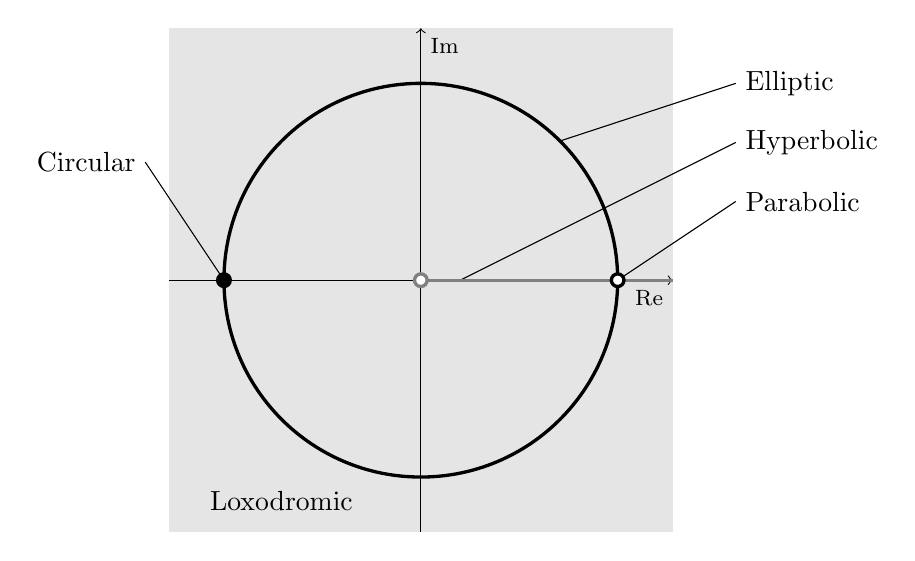
\begin{tikzpicture}

    \fill[gray!20] (-3.2, -3.2) rectangle (3.2, 3.2);

    \draw[very thick] (0, 0) circle (2.5 cm); 
    \draw[->] (-3.2, 0) -- (3.2, 0) node[anchor=north east] {\footnotesize{Re}};
    \draw[->] (0, -3.2) -- (0, 3.2) node[anchor=north west] {\footnotesize{Im}};

    \draw (0.5, 0) -- (4, 1.75) node[anchor=west] {Hyperbolic};
    \draw (2.5, 0) -- (4, 1) node[anchor=west] {Parabolic};
    \draw[gray, very thick] (0, 0) -- (3.2, 0);

    \filldraw[fill=white, very thick] (2.5, 0) circle (0.08 cm);
    \filldraw[fill=black, very thick] (-2.5, 0) circle (0.08 cm);
    \filldraw[color=gray, fill=white, very thick] (0, 0) circle (0.08 cm);

    \node[anchor=west] at (-2.8, -2.8) {Loxodromic};
    \draw (1.7677669529663689, 1.7677669529663689) -- (4, 2.5) node[anchor=west] {Elliptic};

    \draw (-2.5, 0) -- (-3.5, 1.5) node[anchor=east] {Circular};

    \node[anchor=south east] at (3.2, -3.2) {\(\complex\)};

\end{tikzpicture}
 
    \caption{Classification of Möbius transformation in terms of the location of the multiplier \(\kappa\) in the complex plane. Any point that is not on the unit circle yields a loxodromic transformation; a particular subclass consists of the hyperbolic transformations, which are on the real axis except at \(-1\) and \(1\) where it intersects with the unit circle, and at the origin, where the transformation becomes singular. If the multiplier lies on the unit circle (apart from $\kappa = 1$) the transformations are elliptic. A special case is the circular transformation for \(\kappa = -1\). Finally, the parabolic transformations have a multiplier of 1 \cite{Needham1997}.}
    \label{fig:multiplier_regions}
\end{figure}
To summarize, there are five different classes of Möbius transformation: circular, elliptic, hyperbolic, loxodromic, and parabolic. Circular transformations are part of the elliptic transformations and hyperbolic transformations are a subclass of loxodromic transformations. The class to which a Möbius transformation belongs is determined completely by its trace \(a + d\), or equivalently, the value of the multiplier \(\kappa\). For the multiplier, one can distinguish several `regions' in the complex plane that are each associated with a class of Möbius transformations, this is visualized in \cref{fig:multiplier_regions}. The nature of the Jordan form of the matrix associated with a Möbius transformation also clearly gives away to which class a transformation belongs. 
\begin{figure}
    \centering
    \begin{tikzpicture}
    \node at (0, 0) {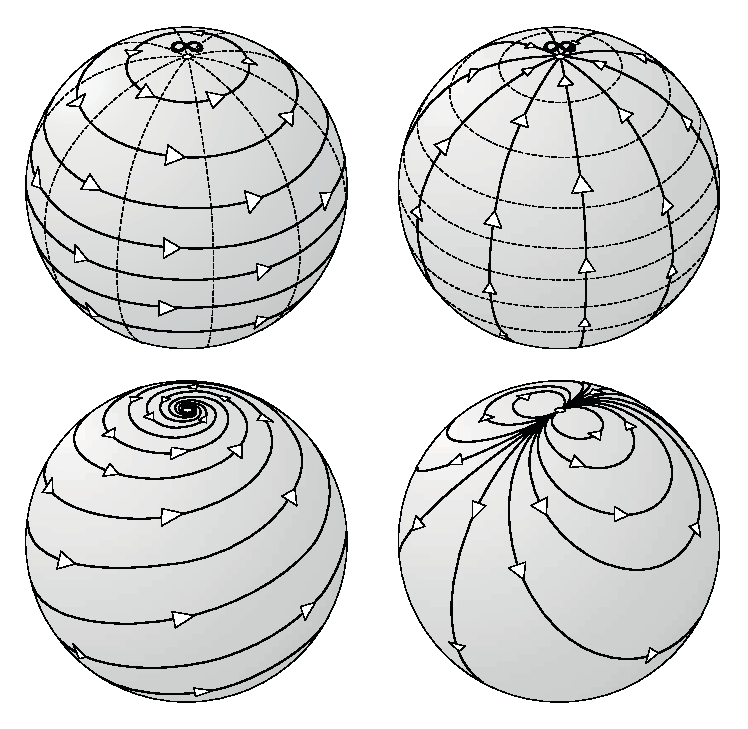
\includegraphics{media/tikz/mobius_transforms_needham.eps}};
    \node at (-3.1, 6.3) {\textbf{Elliptic}};
    \node at (3.2, 6.3) {\textbf{Hyperbolic}};
    \node at (-3.3, -6.3) {\textbf{Loxodromic}};
    \node at (3.3, -6.3) {\textbf{Parabolic}};
    \draw (-6.5, 0) -- (6.5, 0);
    \draw (0, -6.5) -- (0, 6.5);
\end{tikzpicture}

    \caption{Overview of the four classes of Möbius transformation and their typical action on the Riemann sphere. The curves shown on the Riemann sphere are the \emph{invariant curves} of the transformation, i.e. these curves as a whole remain invariant under the transformation. The elliptic, hyperbolic, and loxodromic transformations have the North and South pole, or \(\infty\) and 0 as fixed points, whereas the parabolic transformation only has a single fixed point at the North pole. The loxodromic transformations borrow their name from loxodromes, which are spiral-like trajectories on the Earth with constant bearing --- a ship taking a loxodromic path would maintain a constant angle with respect to true North. Illustration reprinted from \citet[p. 78]{Needham2021}.}
    \label{fig:riemann_transformations}
\end{figure}

\Cref{tab:moebiusclasses} provides an overview of the five Möbius classes, together with the values for the matrix trace, the multiplier, and the Jordan form. Finally, \cref{fig:riemann_transformations} visualizes the effect of each of the transformation classes on points on the Riemann sphere. Elliptic transformations push points along with circles of constant latitude, while hyperbolic transformations move points orthogonally, along the meridians of the Riemann sphere. %Loxodromic transformations are compositions of hyperbolic and elliptic transformations, the associated trajectories therefore look like spirals; incorporating both a North-South and an East-West movement.
\begin{table}
    \caption{Overview of the five classes of Möbius transformations and the corresponding values for the trace squared of the matrix (\(\trace{M} = a + d\)), the multiplier of the transformation, and the Jordan form.}
    \label{tab:moebiusclasses}
    \centering
    \begin{tabular}{lcccc}
        \toprule
        \textbf{Class} & \textbf{Multiplier} & 
        \(\qty(a + d)^2\) & \textbf{Jordan form} & \textbf{Parent class} \\
        \midrule
        Circular    & \(\qty{-1}\)  &  \([0, 4)\) & 
                      \(\mqty(0 & -1 \\ 1 & 0)\) & Elliptic   \\[0.8cm]
        Elliptic    & \(\qty{\kappa \in \complex\;\mid\;\abs{\kappa} = 1, \kappa \neq 1}\)   &  \([0, 4)\) &
                      \(\mqty(\ec^{\theta\ii/2} & 0 \\ 0 & \ec^{-\theta\ii/2})\) & ---  \\[0.8cm]
        Parabolic   & \(\{1\}\)  &  \(\qty{4}\)  & 
                      \(\mqty(1 & b \\ 0 & 1)\) & --- \\[0.8cm]
        Hyperbolic  & \(\real^+_{0} \setminus \qty{1}\) & \((4, +\infty)\)& 
                      \(\mqty(\ec^{\zeta/2} & 0 \\ 0 & \ec^{-\zeta/2})\) & Loxodromic \\[0.8cm]
        Loxodromic  & \(\qty{\kappa \in \complex\;\mid\;\abs{\kappa} \neq 1 }\)  & \(\complex\,\backslash\,[0, 4]\) &
                      \(\mqty(\kappa & 0 \\ 0 & \kappa^{-1})\) & --- \\[0.4cm]
        \bottomrule
    \end{tabular}
\end{table}

\section{Subgroups of the Möbius group}
\label{sec:subgroups}
Apart from the classification considered in the preceding chapter, three subgroups of the Möbius group can be distinguished as well. A compelling observation is that each of these subgroups can each be identified with one of the `geometry types' that were considered in \cref{chap:hyperbolic_geometry}: those of positive (spherical), zero (Euclidean), and negative (hyperbolic) Gaussian curvature. A specific subgroup of the Möbius group will play the role of the direct isometry group on a particular representation of the surfaces that exhibit these geometry types \cite{Needham2021}.

\subsection{Euclidean geometry}
The direct isometries in the Euclidean plane consist simply of translations and rotations. A rotation in the complex plane (around the origin) can be represented simply by \(z \mapsto e^{\ii \theta}\), while a translation is \(z \mapsto z + b\) with \(b \in \complex\). Hence, the entire direct isometry group of the Euclidean plane is given by the particular Möbius transformations of the form
    \[ \mathfrak{E}(z) = e^{\ii\theta} + b. \]
This group is also called the Euclidean group of dimension two.
\index{Euclidean group}

\subsection{Spherical geometry}
A well-known application of group theory in engineering is the representation of rotations in three-dimensional Euclidean space. The group associated with these rotations is the special orthogonal group \(\sogroup\). This group is diffeomorphic to the three-dimensional real projective space \others{\(\mathbb{RP}^3\)}{Three-dimensional real projective space} (intuitively, this space consists of three `directions'). The rotations in \(\real^3\) can be parameterized by \emph{unit quaternions} (also called \emph{versors}): these represent points on the 3-sphere \lsymb{\(\sphere{3}\)}{3-sphere}. The difference between the 3-sphere and the real projective space is that the latter identifies the \emph{antipodal} parts that are present on the sphere. As such, any rotation in \(\real^3\) corresponds precisely to two points on the 3-sphere (or two unit quaternions) --- the group of unit quaternions, therefore, is a double cover of \sogroup. 
\index{real projective space}
\index{quaternions}
\index{versors}
\index{3-sphere}

Quaternions can also be represented as complex matrices: \cite{Stillwell2008}
\[ q = \quat{m}{n}{o}{p} \in \quaternions \corresponds Q = \mqty(m + \ii p & -n - \ii o\\n - \ii o & m - \ii p),\]
which is a general representation of a \(2\times 2\) \emph{unitary}\footnote{A unitary matrix is a matrix whose inverse is its conjugate transpose --- it is the complex counterpart of orthogonal matrices.} matrix. Likewise, the unit quaternions then translate to matrices of the above type with an additional restriction: they must have a determinant of 1: these matrices are members of the \emph{special unitary group} \sugroup{2}. As such, the group of unit quaternions is isomorphic to the \others{\sugroup{2}}{Special unitary group} which is therefore also a double cover of \sogroup.
\index{unitary matrix}

Since the members of \sugroup{2} can be identified with a Möbius transformation (inspection of the matrix above makes this immediately apparent), a specific subgroup of \moebiusgroup can be used to represent the rotations in \(\real^3\) --- recall that every normalized Möbius transformation also corresponds to two matrices, differing by a factor -1. Observing the matrix above, one can see that the entries on the main diagonal are each others' conjugate, while the entries on the antidiagonal are conjugate and opposite. Therefore, the general expression of a rotation of the Riemann sphere as a Möbius transformation can be written as: \cite{Needham2021}
\[\mathfrak{S} = \frac{az + b}{-\conj{b}z+\conj{a}}\quad\text{where } \abs{a}^2 + \abs{b}^2 = 1; \]
the latter equivalent then enforces that \(\det Q = 1\). There are always two quaternions representing the same rotation; they are antipodal and differ by a factor of \(-1\). As a result, there are two possibilities for \(Q\) as well, again identical but with opposite entries. Recall that the same applies to the matrix representations of Möbius transformations: as such, the ambiguities are eliminated, and the group of transformations of type \(\mathfrak{S}\) is isomorphic to \sogroup. In the complex plane, these transformations represent the isometries of spherical geometry in the stereographic map \cite{Needham1997}. 

\index{versor}
\index{quaternion}

\subsection{Hyperbolic geometry}
As described by \citet{Rovenski2010}, the isometries of the Poincaré half-plane (cf. \cref{ssec:poincare_halfplane}) are any (composition) of the following types of transformations, i.e. they leave distances according to the Poincaré metric unaffected:
\begin{itemize}[itemsep=0.3ex,topsep=0.3ex]
    \item horizontal translations: \((x, y)\mapsto(x + a, y)\) where \(x, y, a \in \real\);
    \item reflection around the vertical axis: \((x, y) \mapsto (-x, y)\);
    \item dilations centered around the origin: \((x, y) \mapsto (ax, ay)\);
    \item inversions with respect to the unit circle \(\displaystyle (x, y)\mapsto\qty(\frac{x}{x^2 + y^2},\;\frac{y}{x^2 + y^2})\).
\end{itemize}
The group of all these transformations is precisely \pslgroup{2}{\real}, or the Möbius tranforms with real parameters:
\[\mathfrak{H}(z) = \frac{az + b}{cz + d}\qquad a, b, c, d \in \real \quad ad - bc = 1.\]
These transformations are the isometries of the Poincaré half-plane \cite{Needham2021}. Recall from \cref{ssec:poincare_halfplane} that there are two types of geodesics in the half-plane: semicircles centered at the origin and straight  vertical lines. These are precisely invariant curves for the transformations listed (isometries map geodesics to geodesics) \cite{Lee1997}.

\section{Relation with other groups}
\label{sec:other_groups}
It has been established that the Möbius group as the automorphism group of the Riemann sphere is `trivially' isomorphic to the projective linear group over the complex numbers $\pglgroup{2}{\complex}$, which for this case is identical to the projective special linear group over the complex numbers $\pslgroup{2}{\complex}$. This triviality is due to the fact that the Riemann sphere is equal to the complex projective line. Furthermore, it mentioned in \cref{chap:relativity} that the Möbius group is isomorphic to the restricted Lorentz group $\text{SO}^+(1,3)$. As described by \citet{Needham2021}, the four-vectors from special relativity may be associated with the projective coordinates as follows:
$$
    \mqty(t + z & x + \ii y\\ x - \ii y & t - z) = 2\,\mqty(\mathfrak{z}_1 \\ \mathfrak{z}_2)\mqty(\mathfrak{z}_1 \\ \mathfrak{z}_2)^H,
$$
this is the \emph{spinorial representation} of four-vectors. One can also see this as a parameterization of any vector in the future (positive direction of time) light cone in terms of two complex numbers. The determinant of this matrix coincides with the spacetime interval, which is the quadratic form that the Lorentz transformations must preserve. As such, a Möbius transformation effected on the projective coordinates will preserve this interval as well. It can be shown that this parameterization yields an isomorphism between the Möbius group and the restricted Lorentz group \cite{Penrose1984}. Furthermore, as discussed in \cref{chap:relativity}, the classification of Möbius transformations carries over to the Lorentz transformations too, where hyperbolic elements are Lorentz boosts and elliptic elements are spatial rotations.
\index{spinorial representation}

Another classic Lie group is the special linear group \others{\slgroup{n}{\real}}{Special linear group}, which are the volume-preserving transformations on a vector space --- this property turns out to be quite important. The special linear group over the complex numbers (2-dimensional) \slgroup{2}{\complex} can be represented as the group of all the complex \(2\times2\) matrices with unit determinant. It has been mentioned previously that any such matrix coincides with a Möbius transformation, albeit surjectively: for every Möbius transformation, there are two such matrices. As such, \slgroup{2}{\complex} is a \emph{double cover} of \moebiusgroup.

Arguably more interesting than \slgroup{2}{\complex} is the special linear group over the reals \slgroup{2}{\real}, i.e. every invertible \(2 \times 2\) matrix with real entries and a unit determinant; they form a subgroup of \slgroup{2}{\complex} as well. It has been mentioned before that for the normalized Möbius transformations, the eigenvalues should be complex inverses of each other. For matrices with real entries, the eigenvalues are either both real or complex conjugates of each other. When not on the real axis, the only way eigenvalues can be complex inverses and complex conjugate is to be located on the unit circle. As can be seen on \cref{fig:multiplier_regions}, that means that the matrices with real entries contain exactly the hyperbolic (both real), elliptic (unit circle), and parabolic classes. The remaining part consists of the loxodromic transformations which have a nonreal trace. $\slgroup{2}{\real}$ is in turn isomorphic to two other important groups: the two-dimensional symplectic group \others{$\spgroup{2}$}{Symplectic group} and the special unitary group $\sugroup{1,1}$. As discussed in the previous section, this is the same class of transformations that also constitutes the isometry group of the Poincaré half-plane.
\index{symplectic group}
\index{special unitary group}

Finally, the isomorphisms of the subgroups of the Möbius transformations have been discussed in \cref{sec:subgroups}. Three subgroups can be identified, denoted by $\mathfrak{S}$, $\mathfrak{E}$ and $\mathfrak{H}$, which are respectively isomorphic to the two-dimensional Euclidean group, the three-dimensional rotations ($\sogroup$ covered by the quaternions in $\sugroup{2}$) and the special linear group $\slgroup{2}{\real}$ which also represents the isometries of the Poincaré half-plane.

The relations between the groups are visualized in \cref{fig:group_relations}.

\begin{figure}[h!]
    \centering
    \begin{tikzpicture}
    \node[draw, align=center, thick] (moebius) at (0, 0) {\scriptsize{Möbius group}\\\moebiusgroup = \automorphgroup{\hat{\complex}}};
    \node[draw, align=center] (lorentz) at (0, -2) {\scriptsize{Lorentz group}\\\restlorentzgroup};
    \node[draw, align=center] (psl) at (4, 0) {\scriptsize{Projective special linear group}\\\pslgroup{2}{\complex}};
    \node[draw, align=center] (pgl) at (4, -2) {\scriptsize{Projective linear group}\\\pglgroup{2}{\complex}};

    \node[draw, align=center] (slc) at (0, 4) {\slgroup{2}{\complex}};
    \node[draw, align=center] (slr) at (4, 4) {\slgroup{2}{\real}};

    \node[draw, align=center] (e) at (-4, -2) {\(\mathfrak{E}\)};
    \node[draw, align=center] (s) at (-4, 0) {\(\mathfrak{S}\)};
    \node[draw, align=center] (h) at (3, 1.5) {\(\mathfrak{H}\)};

    \node[draw, align=center] (euclidean) at (-4, -4) {\scriptsize{Euclidean group}};
    \node[draw, align=center] (su) at (-4, 5) {\scriptsize{Special unitary group}\\\sugroup{2}};
    \node[draw, align=center] (so) at (-4, 2) {\scriptsize{Special orthogonal group}\\\sogroup};

    \node[draw, align=center] (su11) at (5, 6) {\scriptsize{Special unitary group}\\\sugroup{1, 1}};
    \node[draw, align=center] (sp) at (1, 6) {\scriptsize{Symplectic group}\\\spgroup{2}{\real}};
    
    \draw[style=double] (moebius) -- (lorentz);
    \draw[style=double] (moebius) -- (psl);
    \draw[style=double] (lorentz) -- (psl);
    \draw[style=double] (lorentz) -- (pgl);
    \draw[style=double] (moebius) -- (pgl);
    \draw[style=double] (pgl) -- (psl);
    \draw[style=double] (s) -- (so);
    \draw[style=double] (e) -- (euclidean);
    \draw[style=double] (su11) -- (sp);
    \draw[style=double] (slr) -- (sp);
    \draw[style=double] (slr) -- (su11);

    \draw[->] (slc) -- (moebius) node[pos=0.5, sloped, anchor=centre, above] {\scriptsize{double cover}};
    \draw[->] (slr) -- (slc) node[pos=0.5, sloped, anchor=centre, above] {\scriptsize{subgroup}};
    \draw[->] (e) -- (moebius) node[pos=0.5, sloped, anchor=centre, above] {\scriptsize{subgroup}};
    \draw[->] (s) -- (moebius) node[pos=0.5, sloped, anchor=centre, above] {\scriptsize{subgroup}};
    \draw[->] (h) -- (moebius) node[pos=0.5, sloped, anchor=centre, above] {\scriptsize{subgroup}};
    \draw[->] (su) -- (so) node[pos=0.5, sloped, anchor=centre, above] {\scriptsize{double cover}};
    \draw[->] (slr) -- (h) node[pos=0.5, sloped, anchor=centre, above] {\scriptsize{double cover}};
\end{tikzpicture}

    \caption{Schematic of the relation of the Möbius group with other important groups such as the special orthogonal group, special unitary group, Lorentz group, etc. Double lines represent isomorphisms, double covers and subgroups are indicated.}
    \label{fig:group_relations}
\end{figure}
\FloatBarrier
\section*{Chapter summary}
Möbius transformations are complex-valued linear fractional transformations. They constitute a group under composition, called the Möbius group. The Möbius group is the automorphism group of the Riemann sphere. The Riemann sphere also represents the complex projective line; the Möbius group can therefore be thought of as the projective linear group over the complex numbers. The Möbius transformations are categorized into five classes: hyperbolic, elliptic, circular, loxodromic and parabolic, based on their conjugacy class in the Möbius group. There are three subgroups of the Möbius group, each of which can be identified as the isometry group (of some representation) of the three geometry types: hyperbolic geometry, spherical geometry and Euclidean geometry. Finally, an isomorphism exists between the restricted Lorentz group and the Möbius group through the spinorial representation of four-vectors.